\title{Sistema de Informação de Solos Brasileiros}
\author{por Stanley Robson de Medeiros, Humberto Gonçalves dos Santos, e Eliane de Paula Clemente}
\maketitle

\newcommand{\SISB}{\href{http://www.bdsolos.cnptia.embrapa.br/consulta_publica.html}{SISB}}

\subsection{Descrição}

O Sistema de Informação de Solos Brasileiros (\SISB) foi desenvolvido com o objetivo de armazenar, gerenciar, recuperar e disponibilizar informações de perfis de solos brasileiros. O banco de dados reúne atributos de solos coletados e analisados de todas as regiões do Brasil, que podem ser acessados via internet. A partir desta base, aplicações podem ser desenvolvidas para auxiliar a tomada de decisões no agronegócio, classificação de solos, zoneamento agrícola, estimativa da produtividade de solos e subsidiar projetos de ensino e pesquisa. A base de dados será continuamente alimentada por pesquisadores da Embrapa e instituições parceiras.

\subsection{Estrutura hierárquica das informações sobre solos}

A principal característica desse sistema é reunir dados de perfis de solos, análises de fertilidade e mapas (\autoref{fig:estrutura}). Os perfis serão úteis, principalmente, para pesquisadores e estudantes da área de Ciência do Solo. Os módulos sobre fertilidade e mapeamento foram idealizados mas ainda não possuem dados, podendo, no futuro subsidiar a tomada de decisões dos agricultores, além do zoneamento agrícola. As informações georreferenciadas complementarão o banco de dados, fornecendo mecanismos de busca eficientes sobre informações de solos disponíveis no território nacional.

\begin{figure*}[tb!]
  \begin{minipage}[t]{\linewidth}
    \centering
    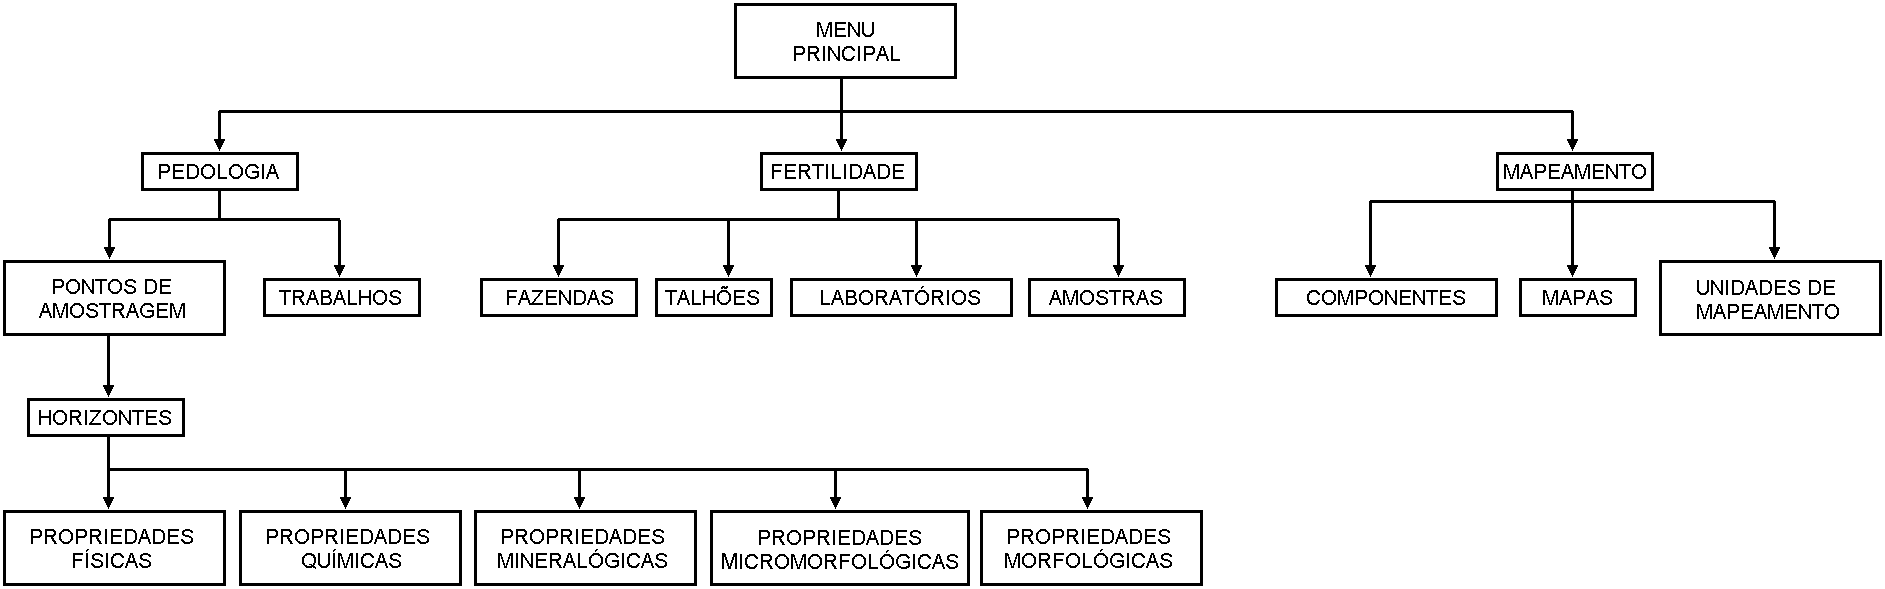
\includegraphics{figuras/estrutura}
    \caption{Estrutura hierárquica do Sistema de Informação de Solos Brasileiros.}
    \label{fig:estrutura}
  \end{minipage}
\end{figure*}

\paragraph{Pedologia} A base de pedologia congrega dados sobre pontos de amostragem (perfis de solos) e é a parte primordial desse sistema de informação. Perfil é a unidade básica de estudo do solo, constituído por seções mais ou menos paralelas à superfície denominadas horizontes ou camadas. Para cada perfil, o sistema armazena informações sobre propriedades físicas, químicas, mineralógicas, morfológicas e micromorfológicas. Informações de física de solos, tais como dados físico - hídricos em geral, densidade do solo, retenção de umidade, micro e macroporosidade, são escassos na base de dados, já que são dados pouco explorados nos levantamentos de solos e nem sempre constituía uma preocupação dos executores de  levantamentos de solos no passado.

\paragraph{Fertilidade} Esta base congrega amostras de solos provenientes de Unidades de Produção Agrícola - UPA - não oriundas de perfis de solos. O módulo de fertilidade foi integrado ao Sistema de Solos com a finalidade de apoiar a tomada de decisões para agricultores.

\paragraph{Mapeamento} Além de mapas, este módulo contém informações sobre Unidades de Mapeamento, que podem ser entendidas como polígonos definidos ou descritos por um critério de relação solo paisagem. Cada Unidade de Mapeamento é composta por um ou mais \textit{Componentes}, que são entidades relativamente homogêneas e identificáveis de uma área, para a qual uma série de valores de propriedades pode ser armazenada. Este módulo de mapeamento não foi completamente desenvolvido e portanto não está disponível no módulo de consulta.

\subsection{Principais benefícios}

Do ponto de vista prático, o sistema será útil para dar suporte à geração de projetos de pesquisa e à tomada de decisões do agronegócio, como, por exemplo, em zoneamento agrícola e em estimativa da produtividade dos solos com base em dados de perfis representativos de classes de solos. No âmbito do ensino e pesquisa, professores, pesquisadores e alunos de pós-graduação podem ser beneficiados com as informações disponíveis no sistema. Além disso, pode-se ressaltar que o uso de dados disponíveis no sistema, serve de base para estudos agronômicos, tais como, mapas de solos, mapas de fertilidade, aptidão agrícola para culturas, zoneamentos climáticos e agroecológicos, dentre outros.

\subsection{Módulo de consultas}

O sistema incorpora amostras e perfis de solos de todo Brasil, apresentando uma descrição detalhada das características morfológicas, físicas, químicas e mineralógicas de perfis representativos, com suas localizações geográficas. Organizadas em um banco de dados único, as informações existentes podem ser facilmente recuperadas, via internet, e utilizadas pelos setores interessados.

\subsection{Sistema Brasileiro de Classificação de Solos – SiBCS}

Os dados armazenados seguem o formato do SiBCS, colaborando para o fortalecimento do sistema de classificação e facilitando a utilização dos dados que estão em formato normatizado e publicado.

\subsection{Parceria}

O Sistema de Informação de Solos Brasileiros é produto da parceria entre a Embrapa Solos e a Embrapa Informática Agropecuária.

\address{Stanley Robson de Medeiros\\
  Embrapa Informática Agropecuária, Campinas, SP\\
  \url{www.embrapa.br/informatica-agropecuaria}\\
  \email{stanley.oliveira@embrapa.br}}

\address{Humberto Gonçalves dos Santos\\
  Embrapa Solos, Rio de Janeiro, RJ\\
  \url{www.embrapa.br/solos}\\
  \email{humberto.santos@embrapa.br}}

\address{Eliane de Paula Clemente\\
  Embrapa Solos, Rio de Janeiro, RJ\\
  \url{www.embrapa.br/solos}\\
  \email{eliane.clemente@embrapa.br}}
%%% Local Variables: 
%%% mode: latex
%%% TeX-master: 5th-edition.tex
%%% End: 